\documentclass[border=15pt, multi, tikz]{standalone}
\usepackage{import}
\usepackage{ctex}% 中文支持
\usepackage{tikz}

\subimport{./}{init}
\usetikzlibrary{positioning}
\usetikzlibrary{3d} %for including external image
\usetikzlibrary{quotes,angles}
\usetikzlibrary{calc}
\usetikzlibrary{decorations.pathreplacing}

\def\DataColor{rgb:blue,5;white,5}
\def\ConvColor{rgb:yellow,5;red,2.5;white,5}
\def\ConvReluColor{rgb:yellow,5;red,5;white,5}
\def\PoolColor{rgb:red,1;black,0.3}
\def\PcColor{rgb:blue,5;red,2.5;white,5}
\def\PcSquashColor{rgb:blue,5;red,5;white,4}
\def\DcColor{rgb:blue,5;green,15}
\def\SumColor{rgb:blue,5;green,15}
% \def\SoftmaxColor{rgb:magenta,5;black,7}

\begin{document}
\begin{tikzpicture}
%%%%%%%%%%%%%%%%%%%%%%%%%%%%%%%
% 图像大小
%%%%%%%%%%%%%%%%%%%%%%%%%%%%%%%
% 图像经过卷积层1后的图像形状为:  torch.Size([16, 128, 254, 254])
% 经过卷积层2后的图像形状为:  torch.Size([16, 64, 125, 125])
% 经过池化层1后的图像形状为:  torch.Size([16, 64, 123, 123])
% 经过卷积层3后的图像形状为:  torch.Size([16, 64, 121, 121])
% 经过卷积层4后的图像形状为:  torch.Size([16, 32, 59, 59])
% 经过池化层2后的图像形状为:  torch.Size([16, 32, 57, 57])
% 经过卷积层5后的图像形状为:  torch.Size([16, 16, 55, 55])
% 经过卷积层6后的图像形状为:  torch.Size([16, 16, 26, 26])
% 经过池化层3后的图像形状为:  torch.Size([16, 16, 24, 24])
% 经过卷积层1后的图像形状为:  torch.Size([16, 16, 22, 22])
% 经过卷积层2后的图像形状为:  torch.Size([16, 16, 9, 9])
% 变换后形状为:  torch.Size([16, 1296])
% 变换后形状为:  torch.Size([16, 128])
% 变换后形状为:  torch.Size([16, 64])

\tikzstyle{connection}=[ultra thick,every node/.style={sloped,allow upside down},draw=\edgecolor,opacity=0.7]
%%%%%%%%%%%%%%%%%%%%%%%%%%%%%%%%%%%%%%%%%%%%%%%%%%%%%%%%%%%%%%%%%%%%%%%%%%%%%%%%%%%%%%%%
%% Data
%%%%%%%%%%%%%%%%%%%%%%%%%%%%%%%%%%%%%%%%%%%%%%%%%%%%%%%%%%%%%%%%%%%%%%%%%%%%%%%%%%%%%%%%
\node[canvas is zy plane at x=0] (temp) at (-4.5,0,0) {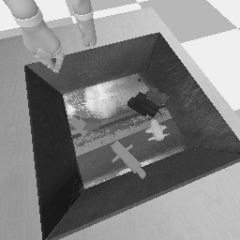
\includegraphics[width=6cm,height=6cm]{observation.png}};
maxpool
% \pic[shift={(-5,0,0)}] at (0,0,0) {Box={name=obs,fill=\DataColor,opacity=0.5,height=32,width=2,depth=32}};
%%%%%%%%%%%%%%%%%%%%%%%%%%%%%%%%%%%%%%%%%%%%%%%%%%%%%%%%%%%%%%%%%%%%%%%%%%%%%%%%%%%%%%%%
%% 卷积单元
%%%%%%%%%%%%%%%%%%%%%%%%%%%%%%%%%%%%%%%%%%%%%%%%%%%%%%%%%%%%%%%%%%%%%%%%%%%%%%%%%%%%%%%%
%% Conv1
\pic[shift={(0,0,0)}] at (0,0,0) {RightBandedBox={name=cr1,%
        xlabel={{"128", "128"}},ylabel=254,zlabel=254,fill=\ConvColor,bandfill=\ConvReluColor,%
        height=60,width=20,depth=60}};
%% Conv2
\pic[shift={(4,0,0)}] at (cr1-east) {RightBandedBox={name=cr2,%
        xlabel={{"64", "64"}},ylabel=125,zlabel=125,fill=\ConvColor,bandfill=\ConvReluColor,%
        height=30,width=12,depth=30}};
% maxpool
\pic[shift={(3,0,0)}] at (cr2-east) {Box={name=p1,fill=\PoolColor,opacity=0.5,height=24,width=2,depth=24}};
% 注释
\node[] at (0, -9, 0) {卷积层1};
\node[] at (8, -5, 0) {卷积层2};
\node[] at (13, -4, 0) {池化层1};
% 卷积单元之间的连接
\draw [connection]  (-4, 0, 0)        -- node {\midarrow} (cr1-west);
\draw [connection]  (cr1-east)        -- node {\midarrow} (cr2-west);
\draw [connection]  (cr2-east)        -- node {\midarrow} (p1-west);
\draw [connection]  (p1-east)        -- node {\midarrow}(15, 0, 0);
% 卷积单元的注释
\draw[decorate, decoration={brace, raise=15pt,amplitude=0.7cm},black!50] (13, -9, 0) -- (0, -9, 0);
\node[] at (6.5, -10.7, 0) {卷积单元};
%%%%%%%%%%%%%%%%%%%%%%%%%%%%%%%%%%%%%%%%%%%%%%%%%%%%%%%%%%%%%%%%%%%%%%%%%%%%%%%%%%%%%%%%
%% 卷积单元需要乘以4
%%%%%%%%%%%%%%%%%%%%%%%%%%%%%%%%%%%%%%%%%%%%%%%%%%%%%%%%%%%%%%%%%%%%%%%%%%%%%%%%%%%%%%%%
\node[canvas is xy plane at z=0] (temp) at (16,0,0) {
\includegraphics[width=2cm,height=2cm]{cellipsis.png}};
\node[canvas is xy plane at z=0] (temp) at (18,0,0) {
\includegraphics[width=2cm,height=2cm]{x3.png}};
\node[canvas is xy plane at z=0] (temp) at (20,0,0) {
\includegraphics[width=2cm,height=2cm]{cellipsis.png}};
%%%%%%%%%%%%%%%%%%%%%%%%%%%%%%%%%%%%%%%%%%%%%%%%%%%%%%%%%%%%%%%%%%%%%%%%%%%%%%%%%%%%%%%%
%% 卷积单元
%%%%%%%%%%%%%%%%%%%%%%%%%%%%%%%%%%%%%%%%%%%%%%%%%%%%%%%%%%%%%%%%%%%%%%%%%%%%%%%%%%%%%%%%
%% Conv1
\pic[shift={(2.5,0,0)}] at (20,0,0) {RightBandedBox={name=cr3,%
        xlabel={{"16", "16"}},ylabel=22,zlabel=22,fill=\ConvColor,bandfill=\ConvReluColor,%
        height=18,width=5,depth=18}};
%% Conv2
\pic[shift={(2,0,0)}] at (cr3-east) {RightBandedBox={name=cr4,%
        xlabel={{"16", "16"}},ylabel=9,zlabel=9,fill=\ConvColor,bandfill=\ConvReluColor,%
        height=15,width=5,depth=15}};

% 注释
\node[] at (22.5, -3.5, 0) {卷积层7};
\node[] at (25.3, -3, 0) {卷积层8};
% 卷积单元之间的连接
\draw [connection]  (21, 0, 0)        -- node {\midarrow} (cr3-west);
\draw [connection]  (cr3-east)        -- node {\midarrow} (cr4-west);
% 卷积单元的注释
\draw[decorate, decoration={brace, raise=15pt,amplitude=0.7cm},black!50] (26, -3.5, 0) -- (22, -3.5, 0);
\node[] at (24, -5, 0) {卷积单元};
% 卷积栈
\draw[decorate, decoration={brace, raise=15pt,amplitude=0.7cm},black!50] (24, -10.5, 0) -- (0, -10.5, 0);
\node[] at (12, -12, 0) {卷积栈};
%%%%%%%%%%%%%%%%%%%%%%%%%%%%%%%%%%%%%%%%%%%%%%%%%%%%%%%%%%%%%%%%%%%%%%%%%%%%%%%%%%%%%%%%
%% Linear Layer1
%%%%%%%%%%%%%%%%%%%%%%%%%%%%%%%%%%%%%%%%%%%%%%%%%%%%%%%%%%%%%%%%%%%%%%%%%%%%%%%%%%%%%%%%
\pic[shift={(4,0,0)}] at (cr4-east) {RightBandedBox={name=fc1-1,
        fill=\PcColor,bandfill=\PcSquashColor,%
        height=8,width=3,depth=3}};
% 平移
\pic[shift={(4,0,4)}] at (cr4-east) {RightBandedBox={name=fc1-2,
        fill=\PcColor,bandfill=\PcSquashColor,%
        height=8,width=3,depth=3}};
\pic[shift={(4,0,4+2)}] at (cr4-east) {RightBandedBox={name=fc1-3,
        fill=\PcColor,bandfill=\PcSquashColor,%
        height=8,width=3,depth=3}};
\pic[shift={(4,0,4+4)}] at (cr4-east) {RightBandedBox={name=fc1-4,
        fill=\PcColor,bandfill=\PcSquashColor,%
        height=8,width=3,depth=3}};
\pic[shift={(4,0,4+6)}] at (cr4-east) {RightBandedBox={name=fc1-5,
        fill=\PcColor,bandfill=\PcSquashColor,%
        height=8,width=3,depth=3}};

\pic[shift={(4,0,-4)}] at (cr4-east) {RightBandedBox={name=fc1-6,
        fill=\PcColor,bandfill=\PcSquashColor,%
        height=8,width=3,depth=3}};
\pic[shift={(4,0,-4-2)}] at (cr4-east) {RightBandedBox={name=fc1-7,
        fill=\PcColor,bandfill=\PcSquashColor,%
        height=8,width=3,depth=3}};
\pic[shift={(4,0,-4-4)}] at (cr4-east) {RightBandedBox={name=fc1-8,
        fill=\PcColor,bandfill=\PcSquashColor,%
        height=8,width=3,depth=3}};
\pic[shift={(4,0,-4-6)}] at (cr4-east) {RightBandedBox={name=fc1-9,
        fill=\PcColor,bandfill=\PcSquashColor,%
        height=8,width=3,depth=3}};
% 省略号
\node[canvas is zy plane at x=0] (temp) at (31,0,2.5) {
\includegraphics[width=2cm,height=2cm]{cellipsis.png}};
\node[canvas is zy plane at x=0] (temp) at (31,0,-1.5) {
\includegraphics[width=2cm,height=2cm]{cellipsis.png}};
% 注释
% \draw[decorate, decoration={brace, raise=15pt,amplitude=0.7cm},black!50] (31, -1, -10) -- (31, -1, 10);
\node[rotate=45] at (27, -6, -2) {1296个元素};
%%%%%%%%%%%%%%%%%%%%%%%%%%%%%%%%%%%%%%%%%%%%%%%%%%%%%%%%%%%%%%%%%%%%%%%%%%%%%%%%%%%%%%%%
%% Draw Dotted Edges 
%%%%%%%%%%%%%%%%%%%%%%%%%%%%%%%%%%%%%%%%%%%%%%%%%%%%%%%%%%%%%%%%%%%%%%%%%%%%%%%%%%%%%%%%
\draw[densely dashed]
    (fc1-5-west)++(3, 3.7, 8) coordinate(a) -- (cr4-nearnortheast)
    (fc1-5-west)++(2, 1.3, 5.5) coordinate(b) -- (cr4-nearsoutheast)
    (fc1-9-west)++(-0.5, -1.9, -3) coordinate(c) -- (cr4-farsoutheast)
    (fc1-9-west)++(0, 1, 0) coordinate(d) -- (cr4-farnortheast)
    ;
%%%%%%%%%%%%%%%%%%%%%%%%%%%%%%%%%%%%%%%%%%%%%%%%%%%%%%%%%%%%%%%%%%%%%%%%%%%%%%%%%%%%%%%%
%% Linear Layer2
%%%%%%%%%%%%%%%%%%%%%%%%%%%%%%%%%%%%%%%%%%%%%%%%%%%%%%%%%%%%%%%%%%%%%%%%%%%%%%%%%%%%%%%%
% 平移
\pic[shift={(8,0,2)}] at (fc1-1-east) {RightBandedBox={name=fc2-1,
        fill=\PcColor,bandfill=\PcSquashColor,%
        height=8,width=3,depth=3}};
\pic[shift={(8,0,2+2)}] at (fc1-1-east) {RightBandedBox={name=fc2-2,
        fill=\PcColor,bandfill=\PcSquashColor,%
        height=8,width=3,depth=3}};
\pic[shift={(8,0,2+4)}] at (fc1-1-east) {RightBandedBox={name=fc2-3,
        fill=\PcColor,bandfill=\PcSquashColor,%
        height=8,width=3,depth=3}};
\pic[shift={(8,0,2+6)}] at (fc1-1-east) {RightBandedBox={name=fc2-4,
        fill=\PcColor,bandfill=\PcSquashColor,%
        height=8,width=3,depth=3}};

\pic[shift={(8,0,-2)}] at (fc1-1-east) {RightBandedBox={name=fc2-5,
        fill=\PcColor,bandfill=\PcSquashColor,%
        height=8,width=3,depth=3}};
\pic[shift={(8,0,-2-2)}] at (fc1-1-east) {RightBandedBox={name=fc2-6,
        fill=\PcColor,bandfill=\PcSquashColor,%
        height=8,width=3,depth=3}};
\pic[shift={(8,0,-2-4)}] at (fc1-1-east) {RightBandedBox={name=fc2-7,
        fill=\PcColor,bandfill=\PcSquashColor,%
        height=8,width=3,depth=3}};
\pic[shift={(8,0,-2-6)}] at (fc1-1-east) {RightBandedBox={name=fc2-8,
        fill=\PcColor,bandfill=\PcSquashColor,%
        height=8,width=3,depth=3}};
% 省略号
\node[canvas is zy plane at x=0] (temp) at (39.4,0,0) {
\includegraphics[width=2cm,height=2cm]{cellipsis.png}};
% 注释
% \draw[decorate, decoration={brace, raise=15pt,amplitude=0.7cm},black!50] (39.4, -1, -8) -- (39.4, -1, 8);
\node[rotate=45] at (36, -5, -2) {128个元素};
%%%%%%%%%%%%%%%%%%%%%%%%%%%%%%%%%%%%%%%%%%%%%%%%%%%%%%%%%%%%%%%%%%%%%%%%%%%%%%%%%%%%%%%%
%% Linear Layer1和Linear Layer2之间的连线
%%%%%%%%%%%%%%%%%%%%%%%%%%%%%%%%%%%%%%%%%%%%%%%%%%%%%%%%%%%%%%%%%%%%%%%%%%%%%%%%%%%%%%%%
% 循环变量
\foreach \from/\to in {fc1-1-east/fc2-1-west, fc1-1-east/fc2-2-west, fc1-1-east/fc2-3-west, fc1-1-east/fc2-4-west, fc1-1-east/fc2-5-west, fc1-1-east/fc2-6-west, fc1-1-east/fc2-7-west, fc1-1-east/fc2-8-west}
    \draw[->]  (\from) -- (\to);
\foreach \from/\to in {fc1-2-east/fc2-1-west, fc1-2-east/fc2-2-west, fc1-2-east/fc2-3-west, fc1-2-east/fc2-4-west, fc1-2-east/fc2-5-west, fc1-2-east/fc2-6-west, fc1-2-east/fc2-7-west, fc1-2-east/fc2-8-west}
    \draw[->]  (\from) -- (\to);
\foreach \from/\to in {fc1-3-east/fc2-1-west, fc1-3-east/fc2-2-west, fc1-3-east/fc2-3-west, fc1-3-east/fc2-4-west, fc1-3-east/fc2-5-west, fc1-3-east/fc2-6-west, fc1-3-east/fc2-7-west, fc1-3-east/fc2-8-west}
    \draw[->]  (\from) -- (\to);
\foreach \from/\to in {fc1-4-east/fc2-1-west, fc1-4-east/fc2-2-west, fc1-4-east/fc2-3-west, fc1-4-east/fc2-4-west, fc1-4-east/fc2-5-west, fc1-4-east/fc2-6-west, fc1-4-east/fc2-7-west, fc1-4-east/fc2-8-west}
    \draw[->]  (\from) -- (\to);
\foreach \from/\to in {fc1-5-east/fc2-1-west, fc1-5-east/fc2-2-west, fc1-5-east/fc2-3-west, fc1-5-east/fc2-4-west, fc1-5-east/fc2-5-west, fc1-5-east/fc2-6-west, fc1-5-east/fc2-7-west, fc1-5-east/fc2-8-west}
    \draw[->]  (\from) -- (\to);
\foreach \from/\to in {fc1-6-east/fc2-1-west, fc1-6-east/fc2-2-west, fc1-6-east/fc2-3-west, fc1-6-east/fc2-4-west, fc1-6-east/fc2-5-west, fc1-6-east/fc2-6-west, fc1-6-east/fc2-7-west, fc1-6-east/fc2-8-west}
    \draw[->]  (\from) -- (\to);
\foreach \from/\to in {fc1-7-east/fc2-1-west, fc1-7-east/fc2-2-west, fc1-7-east/fc2-3-west, fc1-7-east/fc2-4-west, fc1-7-east/fc2-5-west, fc1-7-east/fc2-6-west, fc1-7-east/fc2-7-west, fc1-7-east/fc2-8-west}
    \draw[->]  (\from) -- (\to);
\foreach \from/\to in {fc1-8-east/fc2-1-west, fc1-8-east/fc2-2-west, fc1-8-east/fc2-3-west, fc1-8-east/fc2-4-west, fc1-8-east/fc2-5-west, fc1-8-east/fc2-6-west, fc1-8-east/fc2-7-west, fc1-8-east/fc2-8-west}
    \draw[->]  (\from) -- (\to);
\foreach \from/\to in {fc1-9-east/fc2-1-west, fc1-9-east/fc2-2-west, fc1-9-east/fc2-3-west, fc1-9-east/fc2-4-west, fc1-9-east/fc2-5-west, fc1-9-east/fc2-6-west, fc1-9-east/fc2-7-west, fc1-9-east/fc2-8-west}
    \draw[->]  (\from) -- (\to);
%%%%%%%%%%%%%%%%%%%%%%%%%%%%%%%%%%%%%%%%%%%%%%%%%%%%%%%%%%%%%%%%%%%%%%%%%%%%%%%%%%%%%%%%
%% Linear Layer3
%%%%%%%%%%%%%%%%%%%%%%%%%%%%%%%%%%%%%%%%%%%%%%%%%%%%%%%%%%%%%%%%%%%%%%%%%%%%%%%%%%%%%%%%
% 平移
\pic[shift={(8,0,2)}] at (39.4,0,0) {RightBandedBox={name=fc3-1,
        fill=\PcColor,bandfill=\PcSquashColor,%
        height=8,width=3,depth=3}};
\pic[shift={(8,0,2+2)}] at (39.4,0,0) {RightBandedBox={name=fc3-2,
        fill=\PcColor,bandfill=\PcSquashColor,%
        height=8,width=3,depth=3}};
\pic[shift={(8,0,2+4)}] at (39.4,0,0) {RightBandedBox={name=fc3-3,
        fill=\PcColor,bandfill=\PcSquashColor,%
        height=8,width=3,depth=3}};
\pic[shift={(8,0,-2)}] at (39.4,0,0) {RightBandedBox={name=fc3-4,
        fill=\PcColor,bandfill=\PcSquashColor,%
        height=8,width=3,depth=3}};
\pic[shift={(8,0,-2-2)}] at (39.4,0,0) {RightBandedBox={name=fc3-5,
        fill=\PcColor,bandfill=\PcSquashColor,%
        height=8,width=3,depth=3}};
\pic[shift={(8,0,-2-4)}] at (39.4,0,0) {RightBandedBox={name=fc3-6,
        fill=\PcColor,bandfill=\PcSquashColor,%
        height=8,width=3,depth=3}};
% 省略号
\node[canvas is zy plane at x=0] (temp) at (47.7,0,0) {
\includegraphics[width=2cm,height=2cm]{cellipsis.png}};
% 注释
\node[rotate=45] at (45, -5, -2) {64个元素};
%%%%%%%%%%%%%%%%%%%%%%%%%%%%%%%%%%%%%%%%%%%%%%%%%%%%%%%%%%%%%%%%%%%%%%%%%%%%%%%%%%%%%%%%
%% Linear Layer2和Linear Layer3之间的连线
%%%%%%%%%%%%%%%%%%%%%%%%%%%%%%%%%%%%%%%%%%%%%%%%%%%%%%%%%%%%%%%%%%%%%%%%%%%%%%%%%%%%%%%%
% 循环变量
\foreach \from/\to in {fc2-1-east/fc3-1-west, fc2-1-east/fc3-2-west, fc2-1-east/fc3-3-west, fc2-1-east/fc3-4-west, fc2-1-east/fc3-5-west, fc2-1-east/fc3-6-west}
    \draw[->]  (\from) -- (\to);
\foreach \from/\to in {fc2-2-east/fc3-1-west, fc2-2-east/fc3-2-west, fc2-2-east/fc3-3-west, fc2-2-east/fc3-4-west, fc2-2-east/fc3-5-west, fc2-2-east/fc3-6-west}
    \draw[->]  (\from) -- (\to);
\foreach \from/\to in {fc2-3-east/fc3-1-west, fc2-3-east/fc3-2-west, fc2-3-east/fc3-3-west, fc2-3-east/fc3-4-west, fc2-3-east/fc3-5-west, fc2-3-east/fc3-6-west}
    \draw[->]  (\from) -- (\to);
\foreach \from/\to in {fc2-4-east/fc3-1-west, fc2-4-east/fc3-2-west, fc2-4-east/fc3-3-west, fc2-4-east/fc3-4-west, fc2-4-east/fc3-5-west, fc2-4-east/fc3-6-west}
    \draw[->]  (\from) -- (\to);
\foreach \from/\to in {fc2-5-east/fc3-1-west, fc2-5-east/fc3-2-west, fc2-5-east/fc3-3-west, fc2-5-east/fc3-4-west, fc2-5-east/fc3-5-west, fc2-5-east/fc3-6-west}
    \draw[->]  (\from) -- (\to);
\foreach \from/\to in {fc2-6-east/fc3-1-west, fc2-6-east/fc3-2-west, fc2-6-east/fc3-3-west, fc2-6-east/fc3-4-west, fc2-6-east/fc3-5-west, fc2-6-east/fc3-6-west}
    \draw[->]  (\from) -- (\to);
\foreach \from/\to in {fc2-7-east/fc3-1-west, fc2-7-east/fc3-2-west, fc2-7-east/fc3-3-west, fc2-7-east/fc3-4-west, fc2-7-east/fc3-5-west, fc2-7-east/fc3-6-west}
    \draw[->]  (\from) -- (\to);
\foreach \from/\to in {fc2-8-east/fc3-1-west, fc2-8-east/fc3-2-west, fc2-8-east/fc3-3-west, fc2-8-east/fc3-4-west, fc2-8-east/fc3-5-west, fc2-8-east/fc3-6-west}
    \draw[->]  (\from) -- (\to);
%%%%%%%%%%%%%%%%%%%%%%%%%%%%%%%%%%%%%%%%%%%%%%%%%%%%%%%%%%%%%%%%%%%%%%%%%%%%%%%%%%%%%%%%
%% action
%%%%%%%%%%%%%%%%%%%%%%%%%%%%%%%%%%%%%%%%%%%%%%%%%%%%%%%%%%%%%%%%%%%%%%%%%%%%%%%%%%%%%%%%
\pic[shift={(5,0, 0)}] at (47.7, 0, 0) {Box={name=action-value,fill=\DcColor,%
        height=3,width=3,depth=12}};
% 文字
\node[rotate=45] at (53.7, -1, 0) {机器人最佳执行动作};
%%%%%%%%%%%%%%%%%%%%%%%%%%%%%%%%%%%%%%%%%%%%%%%%%%%%%%%%%%%%%%%%%%%%%%%%%%%%%%%%%%%%%%%%
%% 输出执行动作
%%%%%%%%%%%%%%%%%%%%%%%%%%%%%%%%%%%%%%%%%%%%%%%%%%%%%%%%%%%%%%%%%%%%%%%%%%%%%%%%%%%%%%%%
% 循环变量
\foreach \from/\to in {fc3-1-east/action-value-west}
    \draw[->]  (\from) -- (\to);
\foreach \from/\to in {fc3-2-east/action-value-west}
    \draw[->]  (\from) -- (\to);
\foreach \from/\to in {fc3-3-east/action-value-west}
    \draw[->]  (\from) -- (\to);
\foreach \from/\to in {fc3-4-east/action-value-west}
    \draw[->]  (\from) -- (\to);
\foreach \from/\to in {fc3-5-east/action-value-west}
    \draw[->]  (\from) -- (\to);
\foreach \from/\to in {fc3-6-east/action-value-west}
    \draw[->]  (\from) -- (\to);
\end{tikzpicture}
\end{document}
